\documentclass[12pt]{article}

\usepackage[bottom = 15mm]{geometry}
\usepackage[utf8]{inputenc}
\usepackage[T2A]{fontenc}
\usepackage[russian]{babel}
\usepackage{graphicx}
\usepackage{caption}
\usepackage{amssymb, gensymb, amsmath}
\usepackage{mathrsfs}
\usepackage{array, colortbl}


\textwidth = 16 cm
\textheight = 24 cm
\oddsidemargin = 0 pt
\topmargin = -1.5 cm
\parindent = 20 pt
\parskip = 0 pt
\flushbottom


\title{{\bf Работа 4.\,3.\,2 \\ Дифракция света на ультразвуковой волне в жидкости}}
\author{Лось Денис (группа 611)}
\date{21 февраля 2018}

\begin{document}

\maketitle

\paragraph{Цель работы: } изучение дифракции света на синусоидальной акустической решётке, наблюдение фазовой решётки методом тёмного поля, определение скорости ультразвука в воде, а также периода акустической решётки.

\paragraph{В работе используются: } оптическая скамья, осветитель, два длиннофокусных объектива, кювета с жидкостью, кварцевый излучатель с микрометрическим винтом, генератор ультразвуковой частоты, линза, микроскоп.

\section*{Введение в теоритическую часть}
\par
	При прохождении ультразвуковой волны через жидкость в ней возникают периодические оптические неоднородности, обусловленные разницей значений коэффициента преломления в областях сжатия и разрежения. Эти периодические неоднородности играют роль своеобразной дифракционной решётки для проходящего сквозь жидкость света.
\begin{figure}[h!]
	\centering
	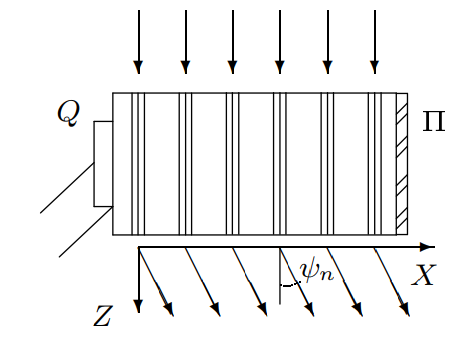
\includegraphics[width = 9cm, height = 5cm]{image1.png}
\end{figure}
\par
	При небольших амплитудах звуковой волны показатель преломления жидкости $n$ меняется по закону
\[
	n = n_0 \left(1 + \alpha \cos Kx \right),
\]
где $K = 2 \pi / \Lambda $ --- волновое число для ультразвуковой волны ($\Lambda$ --- длина ультразвуковой волны), $\alpha$ --- глубина модуляции показателя преломления, определяемая интенсивностью ультразвуковой волны.
\par
	Приняв фазу световых колебаний на передней по ходу лучей поверхности жидкости равной нулю, на задней поверхности ($z = 0$) будем иметь
\[
	\varphi = knL = k n_0 L\left(1 + \alpha \cos Kx \right),
\]
где $L$ --- толщина слоя в кювете. $k$ --- волновое число для света.
\par
	Получается, в плоскости $z = 0$ фаза световых колебаний является периодической функцией координаты, т.е. ультразвуковая волна создаёт в жидкости фазовую дифракционную решётку.
\par
	Для зависимости угла поворота волнового фронта световой волны $\Theta(x)$ от координаты $x$ можем записать:
\[
	\Theta(x) = \frac{dz}{dx} = \frac{1}{k} \frac{d\varphi}{dx} = -Kn_0L \cdot \alpha \sin(Kx) 
\]
\par
	Качественный критерий, при выполнении которого можно пренебречь искривлением световых лучей в кювете, и, следовательно, считать акустическую решётку чисто фазовой:
\[
	|\Theta(x)_\text{max}|L \ll \Lambda \quad \text{или} \quad \alpha \ll \left(\frac{\Lambda}{L} \right)^2
\]
\par
	В случае слабой фазовой модуляции после прохождения через кювету световое поле представимо в виде совокупности трёх, а в общем случае некоторого большого числа плоских волн, которые распространяются под углами, определяемыми из условия
\begin{equation}
	\Lambda \sin\psi_m = m \lambda \quad (m = 0, \pm 1, \pm 2,  \dots) \label{MAIN FR}
\end{equation}
При этом каждая из этих волн соответсвует одному из максимумов в дифракционной картине Фраунгофера.
\newpage
\section*{Наблюдение дифракции на акустической решётке}
\subsection*{Экпериментальная установка}
\par	
	Схема установки для наблюдения дифракции на акустической решётке изображена на рис.1.
\begin{figure}[h!]
	\centering
	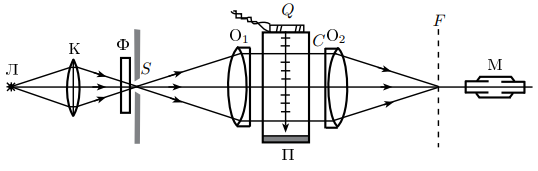
\includegraphics[height = 6cm, width = 15cm]{image2.png}
	\caption{Схема для наблюдения дифракции на акустической решётке}
\end{figure}
\par
	{\bf Источник света Л} через {\bf светофильтр Ф} и {\bf конденсор К} освещает {\bf щель S}, которая расположена в фокусе {\bf объектива ${\bf O_1}$}. Выходящий из объектива параллельный пучок света проходит через {\bf кювету С}, перпендикулярно направлению распространения ультразвуковых волн, которые возбуждаются пьезокварцевой {\bf пластинкой Q}, на которую подаётся напряжение ультразвуковой частоты от генератора. В фокальной плоскости F второго {\bf объектива ${\bf O_2}$} образуется дифракционная картина, наблюдаемая при помощи {\bf микроскопа M}. Пористая резина П в данной установке отсутствует, а следовательно, в кювете образуется стоячая волна, что  позволяет использовать в данной работе метод тёмного поля.
\par
	В данной экспериментальной установке фокусное расстояние объектива $O_2$
\[
	f = 30 \, \text{см}
\]
	В качестве светофильтра Ф используется красный фильтр с полосой пропускания
\[
	\lambda = \left(640 \pm 20\right) \, \text{нм}
\]
\newpage
\subsection*{Методика измерений}
\par
	В силу малости углом $\psi_m$ формула (\ref{MAIN FR}) может быть приведена к виду
\begin{equation}
	l_m = mf \frac{\lambda}{\Lambda}, \label{EQ}
\end{equation}
где $l_m$ --- измеренное на опыте расстояние между $m$-м и нулевым максимумами, а $f$ --- фокусное расстояние объектива $O_2$.
\par
	Соотвественно предлагается измерить положения нескольких дифракционных максимумов $x_m$ c помощью микрометрического винта микроскопа для нескольких частот УЗ-генератора. Построив график зависимости $x_m - x_0$ от порядка $m$ дифракционного максимума, по методу наименьших квадратов найти коэффициент наклона полученной прямой $\beta = \Delta x_m / \Delta m = l_m / m$. 
\par
	Далее для каждой частоты генератора при помощи формулы (\ref{EQ}) найти длину ультразвуковой волны $\Lambda = f \lambda / \beta$. Затем рассчитав для каждой частоты скорость распространения ультразвуковой волны $v = \Lambda \cdot \nu$, где $\nu$ --- частота генератора ультразвуковой частоты, и усреднив полученные результаты, получить искомую скорость ультразвуковой волны $v_\text{уз}$.
\par
	Погрешность коэффициента наклона $\beta$ мы определяем согласно методу наименьших квадратов, принимая во внимание тот факт, что, измеряя $x_m$ c помощью микрометрического винта  c ценой деления 4 мкм, мы будем иметь для них приборную погрешность $\Delta_\text{$x_m$}$, равную 2 мкм. Частоту ультразвукового генератора мы определяем с точностью до $10^{-3}$ МГц.
\par
	Тогда принимая $\sigma$ за обозначение относительной погрешности рассматриваевых величин получим финальные формулы для рассчёта погрешностей
\begin{align*}
	\Delta_\Lambda &= \Lambda \cdot \sqrt{\sigma_\lambda^2 + \sigma_\beta^2} \\
	\Delta_v &= v \cdot \sqrt{\sigma_\lambda^2 + \sigma_\beta^2 + \sigma_\nu^2} \\
	\Delta_\text{$v_\text{уз}$} &= \frac{1}{n} \cdot \sqrt{\Delta_\text{$v_1$}^2 + \dots + \Delta_\text{$v_n$}^2}
\end{align*}
\newpage
\section*{Применение метода тёмного поля}
\subsection*{Экспериментальная установка}
\par
	Чтобы получить видимое изображение фазовой акустической решётки, прежде всего необходимо получить в поле зрения микроскопа изображение задней плоскости (считая по ходу световых лучей) кюветы. Достигнуть этого можно с помошью {\bf вспомогательной линзы ${\bf O}$}, которую необходимо расположить на оптической скамье за фокальной плоскостью объектива $O_2$. Данная схема приведена на рис.2. Остальные элементы и их характеристики, изображённые на рис.2. описаны в пояснении к схеме, изображённой на рис.1. Источник света, светофильтр и конденсор здесь не показаны.
\begin{figure}[h!]
	\centering
	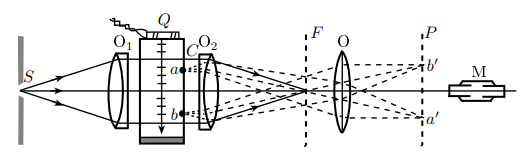
\includegraphics[height = 6cm, width = 13cm]{image3.png}
	\caption{Схема для наблюдения акустической решётки методом тёмного поля}
\end{figure}
\subsection*{Методика измерений}
\par
	Прежде чем приступить непосредственно к методу тёмного поля, необходимо найти цену деления окулярной шкалы микроскопа, которая нам потребуется для дальнейших измерений. Для этого, прижав к задней стенке кюветы стеклянную пластинку с миллиметровыми делениями, совместим её деления с делениями окулярной шкалы и определим количество тех и других делений.
\par
	Далее закрыв центральный максимум вертикальной нитью и убедившись, что после этого в поле зрения видны тёмные и светлые полосы, будем измерять расстояние между самыми дальними из хорошо видимых тёмных полос, а также просчитывать число промежутков между ними. Согласно теории метода тёмного поля расстояние между тёмными полосами соответствует смещению в плоскости кюветы на $\Lambda / 2$. Следовательно, исходя их вышесказанного, длина ультразвуковой волны может быть определена как
\[
	\Lambda = 2 \, \frac{s \cdot \delta_y}{N},
\]
где $s$ --- число делений между самыми дальними из хорошо видимых тёмных полос, $N$ --- число промежутков между ними, а $\delta_y $ --- цена деления окулярной шкалы.
\par
	Приведём соотвествующие формулы для рассчёта погрешностей определения длины ультразвуковой волны, а также её скорости распространения $v_\text{уз}$.
\begin{align*}
	\Delta_\Lambda &= \Lambda \cdot \sigma_s \\
	\Delta_v &= v \cdot \sqrt{\sigma_\Lambda^2 + \sigma_\nu^2} \\
	\Delta_\text{$v_\text{уз}$} &= \frac{1}{n} \cdot \sqrt{\Delta_\text{$v_1$}^2 + \dots + \Delta_\text{$v_n$}^2}
\end{align*}
\section*{Ход работы}
\subsection*{Наблюдение дифракции на акустической решётке}
\begin{table}[h!]
	\centering
	\begin{tabular}{|c|c|}
	\hline
		$l_m$, дел & $m$ \\
	\hline
		0 & 0 \\
	\hline
		39 & 1 \\
	\hline
		81 & 2 \\
	\hline
		121 & 3 \\
	\hline
		-42 & -1 \\
	\hline
		-82 & -2 \\
	\hline
		-123 & -3 \\
	\hline
	\end{tabular}
	\caption{Таблица измерений $l_m$ от $m$ при частоте $\nu = 1.221$ МГц}
\end{table}
\begin{table}[h!]
	\centering
	\begin{tabular}{|c|c|}
	\hline
		$l_m$, дел & $m$ \\
	\hline
		0 & 0 \\
	\hline
		43 & 1 \\
	\hline
		91 & 2 \\
	\hline
		-48 & -1 \\
	\hline
		-92 & -2 \\
	\hline
	\end{tabular}
	\caption{Таблица измерений $l_m$ от $m$ при частоте $\nu = 1.355$ МГц}
\end{table}
\begin{table}[h!]
	\centering
	\begin{tabular}{|c|c|}
	\hline
		$l_m$, дел & $m$ \\
	\hline
		0 & 0 \\
	\hline
		37 & 1 \\
	\hline
		76 & 2 \\
	\hline
		118 & 3 \\
	\hline
		-40 & -1 \\
	\hline
		-76 & -2 \\
	\hline
		-114 & -3 \\
	\hline
	\end{tabular}
	\caption{Таблица измерений $l_m$ от $m$ при частоте $\nu = 1.136$ МГц}
\end{table}
\newpage
\subsection*{Построенные графики}
\begin{figure}[h!]
	\centering
	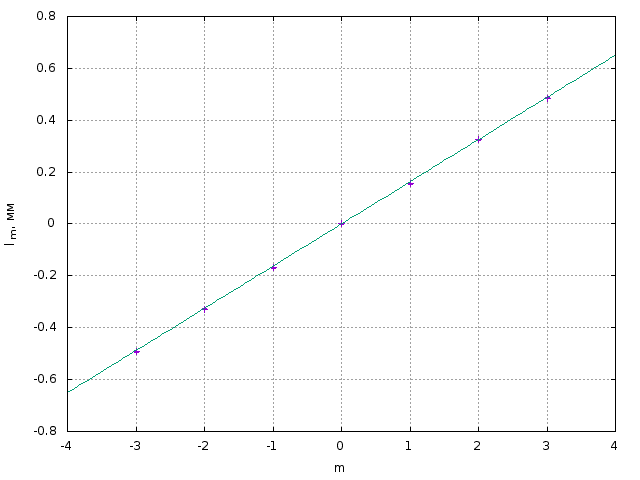
\includegraphics[width = 12cm, height = 7cm]{plot1.png}
	\caption{График зависимости $l_m$ от $m$ при $\nu = 1.221$ МГц}
\end{figure}
\begin{figure}[h!]
	\centering
	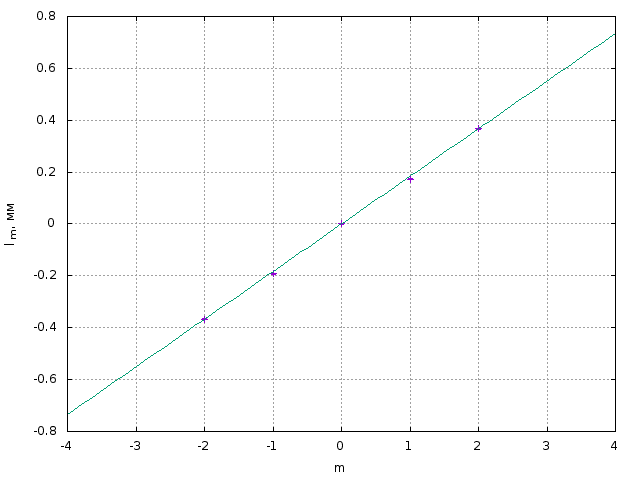
\includegraphics[width = 12cm, height = 7cm]{plot3.png}
	\caption{График зависимости $l_m$ от $m$ при $\nu = 1.355$ МГц}
\end{figure}
\newpage
\begin{figure}[h!]
	\centering
	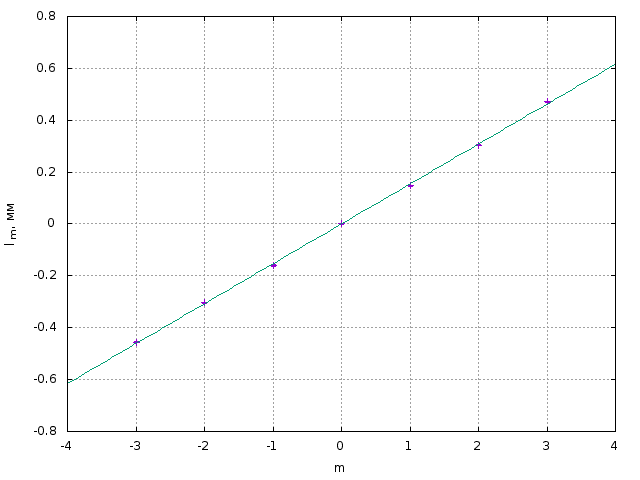
\includegraphics[width = 12cm, height = 7cm]{plot2.png}
	\caption{График зависимости $l_m$ от $m$ при $\nu = 1.136$ МГц}
\end{figure}
\subsection*{Найденные с помощью МНК коэффициенты наклона $\beta$}
\begin{table}[h!]
	\centering
	\begin{tabular}{|c|c|c|c|}
	\hline
		$\nu$, МГц & $\beta$, мм & $\Delta_\beta$, мм & $\sigma_\beta$, \% \\
	\hline
		1.221 & 0.1627 & 0.0009 & 0.6 \\
	\hline
		1.355 & 0.1840 & 0.003 & 1.6 \\
	\hline
		1.136 & 0.1539 & 0.0012 & 0.8 \\
	\hline
	\end{tabular}
\end{table}
\subsection*{Рассчитанные длины УЗ-волн для каждой из частот}
\begin{table}[h!]
	\centering
	\begin{tabular}{|c|c|c|c|c|c|}
	\hline
		$\nu$, МГц & $\Lambda$, мм & $\Delta_\Lambda$, мм & $\sigma_\Lambda$, \% & $v$, м / c & $\Delta_v$, м / c \\
	\hline
		1.221 & 1.18 & 0.04 & 3.4 & 1441 & 49 \\  
	\hline
		1.355 & 1.04 & 0.04 & 3.8 & 1414 & 54 \\ 
	\hline
		1.136 & 1.24 & 0.04 & 3.2 & 1417 & 45 \\
	\hline
	\end{tabular}
\end{table}
\par
	В результате получившаяся скорость распространения ультразвуковой волны в воде
\[
	v_\text{уз} = \left(1420 \pm 30 \right) \, \frac{\text{м}}{\text{c}}
\]
\newpage
\subsection*{Применение метода тёмного поля}
\subsection*{Калибровка окулярной шкалы микроскопа}
\par
	Принимая за $a$ --- число делений миллиметровой пластинки, $b$ --- число делений окулярной шкалы микроскопа, а за $\delta_y$ --- цену деления окулярной шкалы, получим
\begin{table}[h!]
	\centering
	\begin{tabular}{|c|c|}
	\hline
		$a$, дел & $b$, дел \\
	\hline
		13 & 170 \\
	\hline
	\end{tabular}
\end{table}
\par
	А следовательно, $\delta_y = 76$ мкм.
\paragraph{Определение длины и скорости распространения ультразвуковой волны методом тёмного поля} 
\par
	Принимая за $s$ --- расстояние между самыми дальними их хорошо видимых в поле зрения тёмных полос, а за $N$ --- число промежутков между ними, получим
\begin{table}[h!]
	\centering
	\begin{tabular}{|c|c|c|c|c|c|c|c|}
	\hline
		$\nu$, МГц & $s$, дел & $N$ & $\Lambda$, мм & $\Delta_\Lambda$, мм & $\sigma_\Lambda$, \% & $v$, м / c & $\Delta_v$, м / c \\
	\hline
		1.187 & 162 & 20 & 1.231 & 0.008 & 0.6 & 1461 & 9 \\
	\hline
		1.292 & 145 & 19 & 1.160 & 0.008 & 0.7 & 1498 & 9 \\
	\hline
		1.437 & 150 & 22 & 1.036 & 0.007 & 0.7 & 1489 & 10 \\
	\hline
	\end{tabular}
\end{table}
\par
	В результате получившаяся скорость распространения ультразвука в воде, найденная с помощью метода тёмного поля
\[
	v_\text{уз} = \left(1483 \pm 5 \right) \, \frac{\text{м}}{\text{c}}
\]
\section*{Выводы}
\par
	В ходе работы нам удалось пронаблюдать явление дифракции световой волны на акустической решётке, создаваемой ультразвуковой волной в воде. Также мы наблюдали непосредственно саму фазовую решётку, используя для этого метод тёмного поля. Как в ходе наблюдения дифракции, так и в ходе наблюдения акустической решётки с помощью метода тёмного поля нами были получены длина ультразвуковой волны при различных частотах, а также скорость распространения ультразвуковой волны в воде. Приведём повторно полученные результаты
\begin{align*}
	v_\text{зв дифр} &= \left(1420 \pm 30\right) \, \frac{\text{м}}{\text{c}} \\
	v_\text{зв т. поле} &= \left(1483 \pm 5\right) \, \frac{\text{м}}{\text{c}} \\
\end{align*}
\par
	Полученные результаты согласуются с известным табличным значением для скорости распространения ультразвуковой волны в воде
\[
	v_\text{табл} = 1481 \, \frac{\text{м}}{\text{c}}
\]
\end{document}